\section{Results and Evaluation}
The Results section is dedicated to presenting the actual results (i.e. measured and calculated quantities), not to discussing their meaning or interpretation.
The results should be summarized using appropriate Tables and Figures (graphs or schematics).
Every Figure and Table should have a legend that describes concisely what is contained or shown.
Figure legends go below the figure, table legends above the table.
Throughout the report, but especially in this section, pay attention to reporting numbers with an appropriate number of significant figures.


\begin{table}[ht]
\begin{tabular}{|l|l|l|l|l|}
\hline
                    & Test accuracy   & Test F1 & Test Loss \\ \hline
CNN                 & \textbf{0.3975} & 0.2414  & 3.7596    \\ \hline
CNN augmented       & 0.2825          & 0.2414  & 6.2656    \\ \hline
Tuned CNN           & 0.3900          & 0.2414  & 2.3860    \\ \hline
Tuned CNN augmented & 0.3787          & 0.2414  & 2.0166    \\ \hline
\end{tabular}
\end{table}

\begin{table}[ht]
\begin{tabular}{|l|l|l|l|}
\hline
                    & Train accuracy & Train F1 & Train Loss \\ \hline
CNN                 & 0.9998         & 0.2414   & 0.0011     \\ \hline
CNN augmented       & 0.9939         & 0.2414   & 0.0172     \\ \hline
Tuned CNN           & 0.9998         & 0.2414   & 0.0065     \\ \hline
Tuned CNN augmented & 0.8073         & 0.2414   & 0.6131     \\ \hline
\end{tabular}
\end{table}

\begin{table}[ht]
\begin{tabular}{|l|l|l|l|}
\hline
                    & Validation accuracy & Validation F1 & Validation Loss \\ \hline
CNN                 & 0.4663              & 0.2414        & 2.9336          \\ \hline
CNN augmented       & 0.3988              & 0.2414        & 5.8118          \\ \hline
Tuned CNN           & 0.4175              & 0.2414        & 2.0767          \\ \hline
Tuned CNN augmented & 0.4450              & 0.2414        & 1.7493          \\ \hline
\end{tabular}
\end{table}

\begin{figure}[ht]
\centering
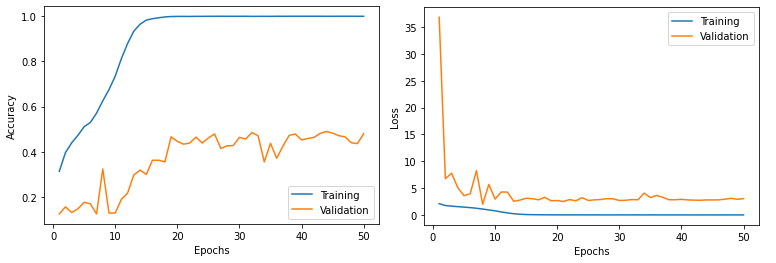
\includegraphics[scale=0.6]{images/2021-val-train.png}
\caption{CNN's Accuracy and Loss function of the training and validation set.}
\label{fig:Acc_Loss_2021}
\end{figure}

\begin{figure}[ht]
\centering
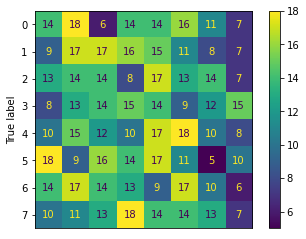
\includegraphics[scale=0.6]{images/2021-confusion_matrix.png}
\caption{CNN's confusion matrix.}
\label{fig:cf_2021}
\end{figure}

\begin{figure}[ht]
\centering
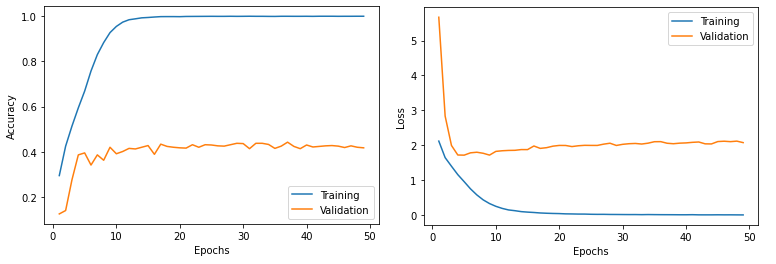
\includegraphics[scale=0.6]{images/tuned-val-train.png}
\caption{Tuned CNN's Accuracy and Loss function of the training and validation set.}
\label{fig:Acc_Loss_tuned}
\end{figure}

\begin{figure}[ht]
\centering
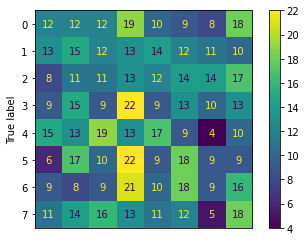
\includegraphics[scale=0.6]{images/tuned-confusion_matrix.png}
\caption{Tuned CNN's confusion matrix.}
\label{fig:cf_tuned}
\end{figure}

\begin{figure}[ht]
\centering
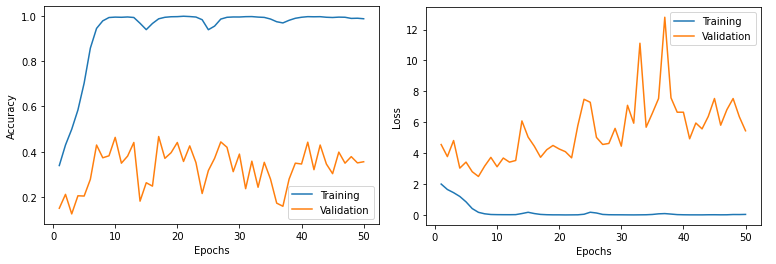
\includegraphics[scale=0.6]{images/aug-2021-val-train.png}
\caption{CNN's Accuracy and Loss function of the training and validation set with data augmentation.}
\label{fig:Acc_Loss_2021_aug}
\end{figure}

\begin{figure}[ht]
\centering
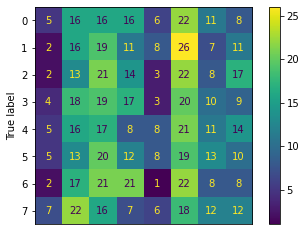
\includegraphics[scale=0.6]{images/aug-2021-confusion_matrix.png}
\caption{CNN's confusion matrix with data augmentation.}
\label{fig:cf_2021_aug}
\end{figure}

\begin{figure}[ht]
\centering
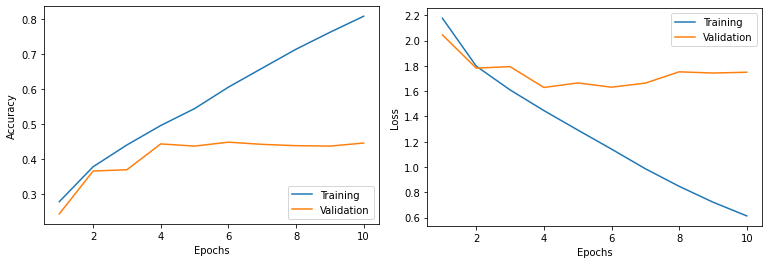
\includegraphics[scale=0.6]{images/aug-tuned-val-train.png}
\caption{Tuned CNN's Accuracy and Loss function of the training and validation set with data augmentation.}
\label{fig:Acc_Loss_tuned_aug}
\end{figure}

\begin{figure}[ht]
\centering
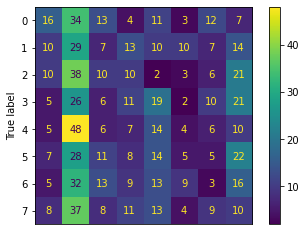
\includegraphics[scale=0.6]{images/aug-tuned-confusion_matrix.png}
\caption{Tuned CNN's confusion matrix with data augmentation.}
\label{fig:cf_tuned_aug}
\end{figure}